\documentclass{article}
\usepackage{amsmath}
\usepackage{tikz}
\usetikzlibrary{arrows.meta}

\begin{document}

\begin{center}
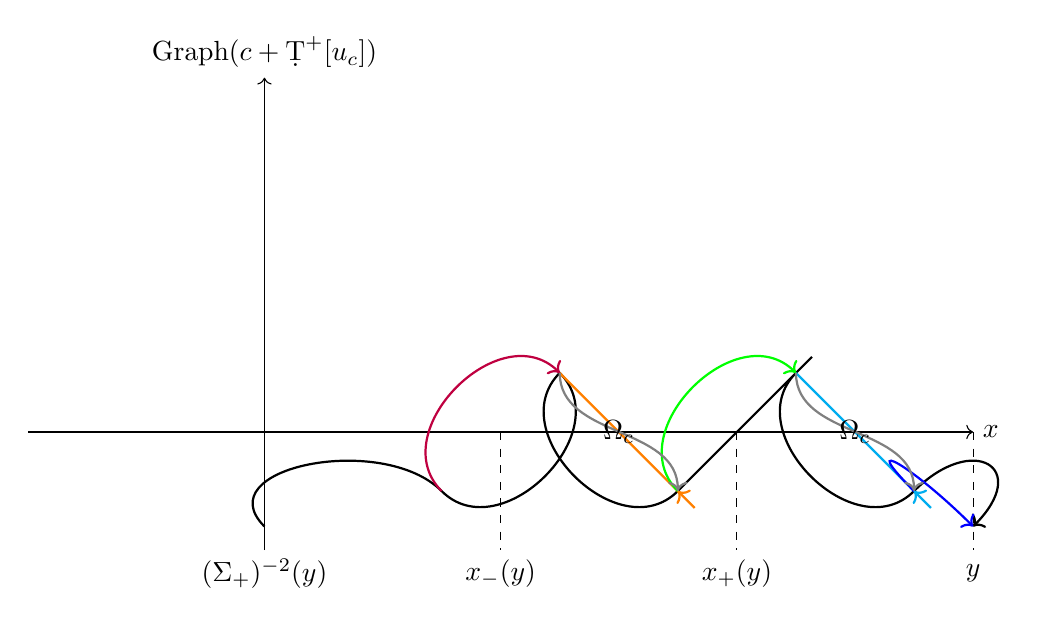
\begin{tikzpicture}[scale=1.5]
    % Axes
    \draw[->] (-2,0) -- (6,0) node[right] {$x$};
    \draw[->] (0,-1) -- (0,3) node[above] {$\operatorname{Graph}(c+\d T^{+}[u_c])$};

    % Dotted lines
    \draw[dashed] (0,0) -- (0,-1);
    \draw[dashed] (2,0) -- (2,-1);
    \draw[dashed] (4,0) -- (4,-1);
    \draw[dashed] (6,0) -- (6,-1);

    % Labels for dotted lines
    \node at (0,-1.2) {$(\Sigma_+)^{-2}(y)$};
    \node at (2,-1.2) {$x_{-}(y)$};
    \node at (4,-1.2) {$x_{+}(y)$};
    \node at (6,-1.2) {$y$};

    % Curves
    \draw[thick, black, ->] (0,-0.8) .. controls +(-0.5,0.5) and +(-0.5,0.5) .. (1.5,-0.5) .. controls +(0.5,-0.5) and +(0.5,-0.5) .. (2.5,0.5) .. controls +(-0.5,-0.5) and +(-0.5,-0.5) .. (3.5,-0.5) .. controls +(0.5,0.5) and +(0.5,0.5) .. (4.5,0.5) .. controls +(-0.5,-0.5) and +(-0.5,-0.5) .. (5.5,-0.5) .. controls +(0.5,0.5) and +(0.5,0.5) .. (6,-0.8);
    
    \draw[thick, purple, ->] (1.5,-0.5) .. controls +(-0.5,0.5) and +(-0.5,0.5) .. (2.5,0.5);
    \draw[thick, orange, ->] (2.5,0.5) .. controls +(0.5,-0.5) and +(0.5,-0.5) .. (3.5,-0.5);
    \draw[thick, green, ->] (3.5,-0.5) .. controls +(-0.5,0.5) and +(-0.5,0.5) .. (4.5,0.5);
    \draw[thick, cyan, ->] (4.5,0.5) .. controls +(0.5,-0.5) and +(0.5,-0.5) .. (5.5,-0.5);
    \draw[thick, blue, ->] (5.5,-0.5) .. controls +(-0.5,0.5) and +(-0.5,0.5) .. (6,-0.8);

    % Arrows for the map Omega_c
    \draw[->, thick, gray] (2.5,0.5) to[out=-90,in=90] (3.5,-0.5);
    \node at (3,0) {$\Omega_c$};
    \draw[->, thick, gray] (4.5,0.5) to[out=-90,in=90] (5.5,-0.5);
    \node at (5,0) {$\Omega_c$};
\end{tikzpicture}
\end{center}

\end{document}